\documentclass[main.tex]{subfiles}
\begin{document}

\chapter{Life emerges...}

\newpara \nar For a long while, there was only darkness.  Well, mostly darkness.  Photons are to the Universe what bacteria are to the world.  In a nutshell, that stuff is \textit{everywhere}.  

\newpara \nar But on a very fateful day, everything changed.  Cosmic Dawn emerges with a roar.  All due to an especially massive Giant Molecular Cloud in the final stages of contracting; the internal pressure from within, supported by the random motions of Her constituent atoms and molecules, is finally losing out to the inward and unrelenting pull of gravity.  Over-dense knots and filaments begin to form within Her belly.  The knots continue to coalesce, becoming ever hotter and denser. Until, finally, new life emerges.  

\newpara \nar With their birth, comes Dawn.  Protostars spew out photons at a thunderous pace; enough to dwarf an unfathomable mound of radioactive waste.  Seven siblings, all born within the narrow window of a million years. Their Mother, \rmpleione, a particularly compelling Giant Molecular Cloud, now begins her journey through Motherhood.  But it's not yet over; she's still in the process of yielding to gravity's nurturing might, slowly contracting and compressing, forming over-dense filaments and birthing new stars within her bossom.  

\newpara \Maia Hello to you, Mother!\footnote{Stars of course cannot speak.  But they can communicate with each other, even over very large distances.  They communicate by modulating their luminosities on short timescales, brightening and dimming, brightening and dimming, in whatever cadence properly communicates their intended message.  Humans are unable to speak, write or even read the language of the stars.  Throughout this book, all communications between stars will be expressed in English.} 

\newpara \Pleione Hello to you as well, my child.  My young new protostar.

\newpara \Maia Wow!  The Universe is so amazing and pretty.  Are all those twinkling things off in the distance other protostars, like me?

\newpara \Pleione Mostly no, child.  Stars live long lives, and the protostellar phase does not last long; only a few million years.  Most of the far off stars you are looking at are much older than you.

\newpara \Maia Gotcha.  Long lives.  I'll take it!  Whoa, if you look closely at some of the stars, they appear to be arranged in interesting ways that make them resemble familiar things.  Like, over there, I see three stars are close together that form a straight line.

\newpara \Pleione That is Orion's Belt, good eye!  If you take a larger look at him, you will notice as well a torso, arms and legs.  

\newpara \Maia Ah yes!  I see them.  

%\newpara \nar \rmmaia~ proceeded to elaborately describe her interpretation of Orion the Hunter (see Figure~\ref{fig:fig1}).

%\newpara \Pleione You are close child, but it is supposed to look more like this (see Figure~\ref{fig:fig1}).

%\begin{figure}
%\begin{center}
%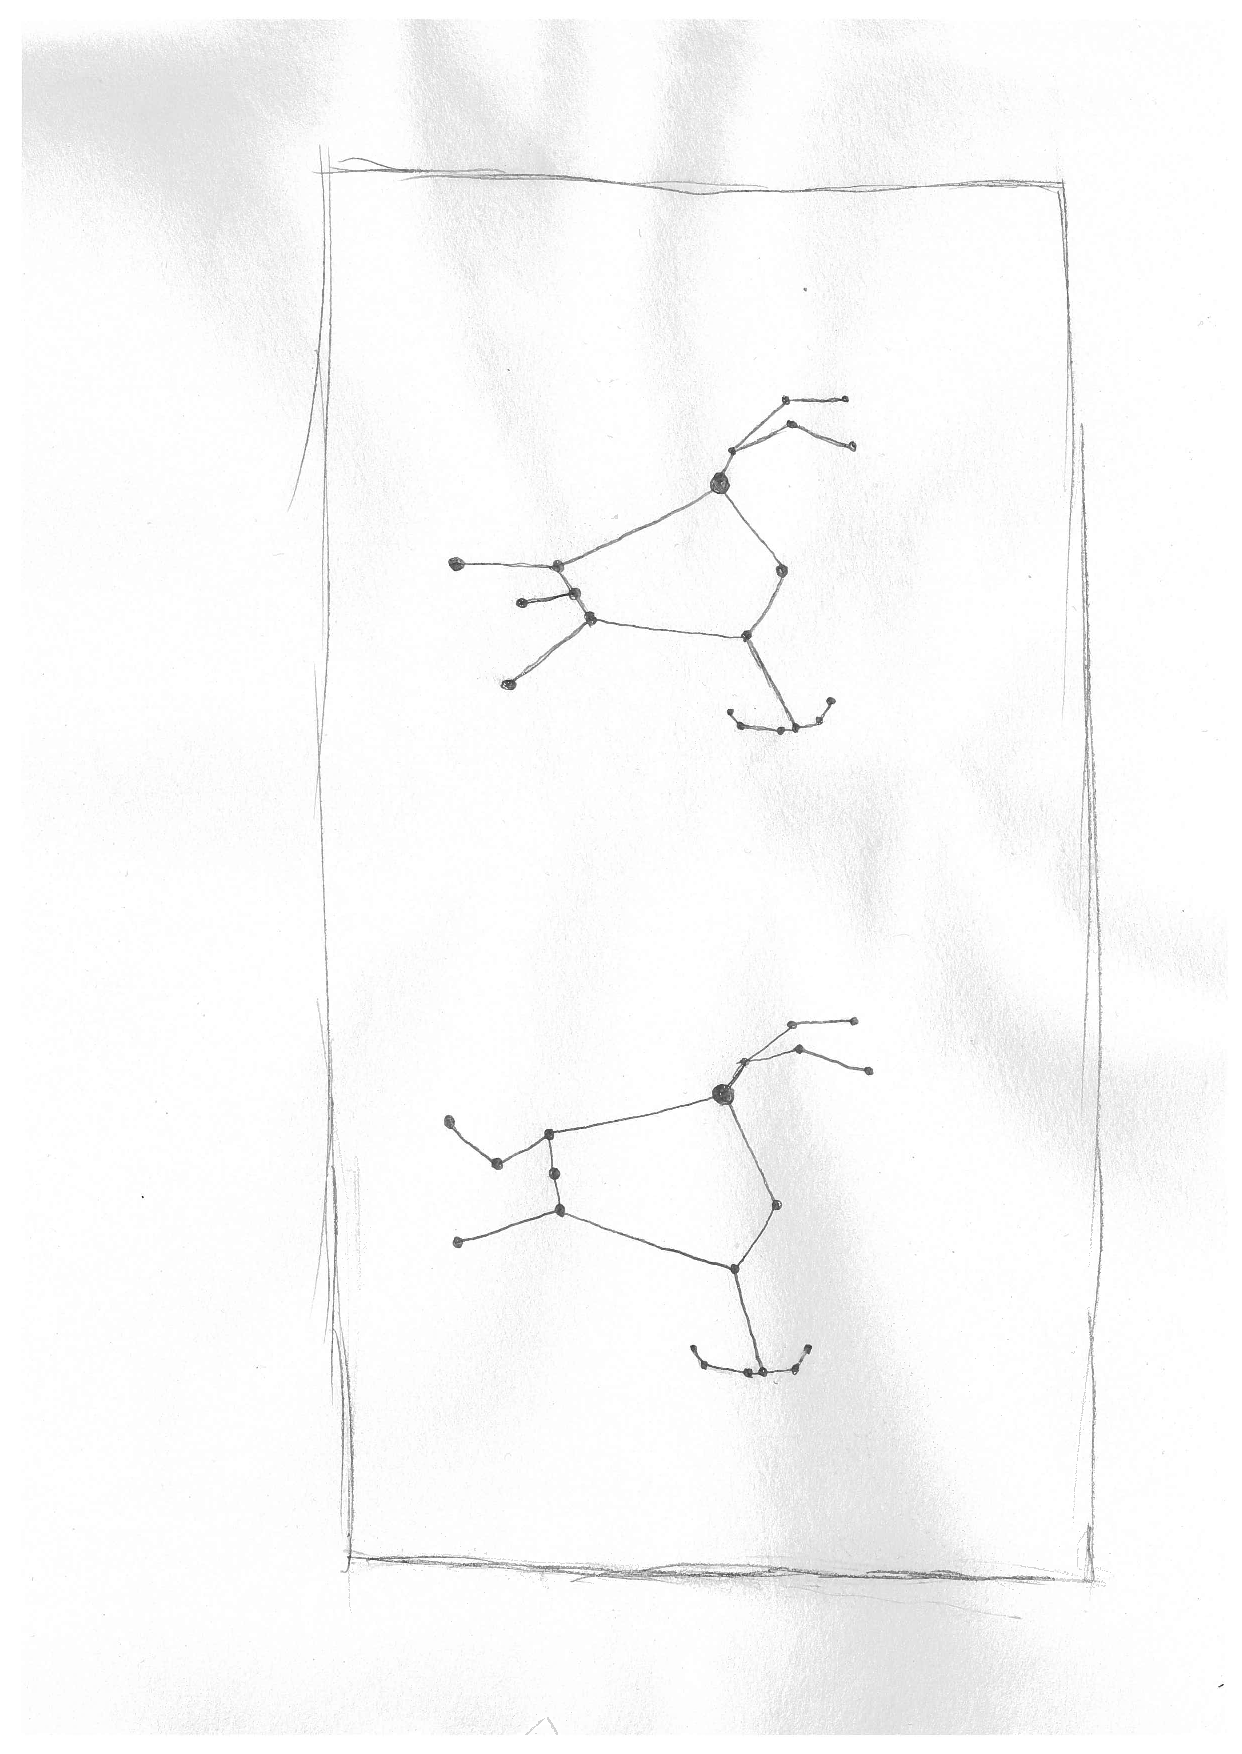
\includegraphics[width=\columnwidth]{Orion.eps}
%\end{center}
%\caption[Schematic depictions of Orion the Hunter]{Left panel:  \rmmaia's interpretation of the constellation Orion the Hunter.  Right panel:  \rmpleione's corrected version of the constellation Orion the Hunter.
%\label{fig:fig1}}
%\end{figure}

%\newpara \Maia Oh okay.  He only has two legs then.  I wasn't sure.

%\newpara \Pleione Oooooh!  That is supposed to be a leg.  I shouldn't have expected you to know that humans have only two legs.  After all, you've never seen one.

\newpara \Pleione Orion the Hunter is in the form of a human.  He is but one example of the many stories depicted in the night sky, assigned by that species.  They call themselves humans, and dub these familiar stellar configurations ``constellations''.  Humans have developed many stories to explain their origins.

\newpara \Maia Have you ever seen one?

\newpara \Pleione What?

\newpara \Maia A human.

\newpara \Pleione Yes, once, quite some time back.  Awful, vile species.  Constantly littering space with their garbage.

\newpara \Maia Yuck.  That does sound gross.  
%Well, I thought the third leg should be shorter because it's supposed to be back a bit, and I thought that gives it a 3-dimensional feel.  What did \textit{you} think it is?

%\newpara \Pleione Uh... Hey! 
\newpara \Pleione Did you know that Orion the Hunter even has a bow to fire arrows at his enemies?!  If you look closely, you can see he is holding it in his left hand, and it forms a large arc in the sky.

\newpara \Maia Enemies?  What kinds of enemies?

\newpara \Pleione Well, if you follow Orion's Belt from left to right, you will pretty quickly notice a very bright red star.  That is the star \rmaldebarran, the Eye of Taurus the Bull.  As the myth goes, Orion the Hunter fought Taurus the Bull to save the Seven Sisters.  

\newpara \Maia Wow, that sounds very dramatic.

\newpara \rmpleione~ was growing weary, having now birthed many stars.  Each of her children emitting a wind of charged particles and photons escaping wildly from their surface; $>$ 10$^{38}$ bats out of Hell every second.\footnote{This estimate comes from assuming that every photon escaping from the surface of the Sun has an energy of 12.86 Mev, corresponding to the highest energy photons produced at the end of the proton-proton-chain (thus our estimate here for the total number of photons should be regarded as a strict lower limit), which is the nuclear reaction process resonsible for converting hydrogen in to helium.  We adopt a solar luminosity of 3.828 $\times$ 10$^{26}$ J s$^{-1}$ for this calculation.}  As the winds collide with the loving embrace of their Mother, she disperses.  Her gas tendrils, swirling and coalescing around her children, gently touching and massaging their young faces, begin to dissipate.

\newpara \Maia Wait, Mother, where are you going?  

\newpara \nar \rmmaia, the second most massive of her soon-to-be-born siblings, wears a worried expression upon her face that begets deep concern for her fleeting Mother.  

%\Maia And why is the entire Universe spinning?  Ugh... I think I might be sick.

%\Mother My child, it is not the Universe that spins, but you.  All stars are born rotating, and you are no excpetion.  But fear not, you were also born with a magnetic field, and this will spin you down over the next several tens of millions of years.

%\Maia Oh, thank goodness.  For a second there, I was worried I would be rapidly rotating forever.  That's a relief.  But, wait, back to where you are going...? 

%\Maia Mother!  Mother!  Don't go!

\newpara \Pleione Oh, young one.  I am now you, inside you always, no matter what adventures befall you.  Please, take me with you, with an open heart.

\newpara \Maia That sounds suspiciously like a goodbye...

\newpara \Pleione Shhhh little one.  Your job is not yet done.  You are only just now born and still contracting, as gravity continues to find its balance with the fires that now rage within you.  Hydrostatic equilibrium awaits.\footnote{Hydrostatic equilibrium is what ultimately decides the size or radius of a star.  The term refers to the balance between the outward pressure supplied by the energy released in the core via nucelar reactions (e.g., the proton-proton-chain, which is what burns hydrogen into helium) and the inward pull of gravity.}

\newpara \Maia Um... You're leaving me with a complicated technical term...?  What does that even mean?

\newpara \Pleione It means that the fires that rage within must balance the forces of the outside world, to ensure stability.  Take care of your siblings, loved one.

\newpara \Maia Uh... Okay...  Still kind of confused over here...

\newpara \nar Just then, one of \rmmaia's siblings awakens.  \rmelectra~ emits a long, sleepy yawn.

\newpara \Pleione Behold!  Your sister awakens!

\newpara \Electra  Uh... Hi.

\newpara \Maia She \textit{is} awful shiny.  It hurts my eyes if I stare right at her... Wait, \textit{is} this hurting my eyes?  Like, could I go blind?

\newpara \Pleione Only if you look directly at her.

\newpara \Maia But I already did that!

\newpara \Pleione Are you blind yet?

\newpara \Maia I don't think so.  

\newpara \Pleione How can you be sure?

\newpara \Maia Well, I can see you wincing, for one thing.  You are looking at me as if I just got in to a fight with a black hole and lost.

\newpara \Pleione Uh... I'm sure you'll be fine. 

\newpara \Maia That was less than convincing.

\newpara \nar \rmelectra~ interrupts them suddenly, belching loudly.  Plasma is ejected from her surface, emanating from above the equator.  

\newpara \nar \rmpleione~ bestows one last kiss upon her daughters, before floating off and dispersing in to the infinite vacuum.

\newpara \Electra It looks to be a lovely day we have on our hands here. ...I feel as though I just missed something important.  Please do fill me in at your earliest convenience.  Wait, what are those two whispering about?

\newpara \nar Both \rmmaia~ and \rmelectra~ turn their gaze toward \rmtaygete~ and \rmalcyone~, who together form a compact binary star system.  Gravitationally bound, the sisters orbit their mutual center of mass in harmony.  Needless to say, they were close.  \rmtaygete~ and \rmalcyone~ quietly conferred about the topic at hand.

\newpara \Taygete I think it goes without saying that I am brighter than you are.

\newpara \Alcyone Dream on!  I outshine you for sure.

\newpara \Taygete Alright, tough guy.  Want to know how I know that I am brighter than you are?

\newpara \Alcyone Sure.  Amuse me.

\newpara \Taygete I'm definitely fatter than you are, and bigger.  Both contribute to making me brighter, relative to \textit{you}.\footnote{The luminosity of a star increases steeply with both increasing mass and radius.  This is the case during the main-sequence phase of a star's life, during which time stars are burning hydrogen into helium in their cores.}  

\newpara \Alcyone Oh shut up...  You are neither fatter nor bigger than I am.  You \textit{are} way more delusional than I am though, I'll give you that.

\newpara \nar \rmtaygete~ and \rmalcyone~ begin flailing at each other violently, intent on a fight.  But they lie outside of each other's grasp; a sisters' quarrel unrealized.  Their efforts futile, they quickly give up.  

\newpara \nar \rmtaygete~ and \rmalcyone~ are in fact two members of a triplet.  The third companion, \rmcelaeno, lies much farther away than the other two, and is often ridicouled by her fellow twins because of it.  But this distance is absolutely necessary to ensure the long-term dynamical stability of the triple;  if the inner pair becomes too wide, the gravity exerted by the outer object pulls them apart.  Chaos ensues; all Hell breaks loose.  This chaos can mediate the ejection of one or more stars from the triple, and even direct collisions.  The triplets' current configuration, hierarchical and dynamically stable, is nothing short of fate; binding them to each other practically indefinitely.

\newpara \Maia Well, I think you are almost certainly identical twins.  I cannot see any real difference between you.  I mean, look at $\rmcelaeno$ out there; she's blue, whereas the two of you are clearly more of a yellow color.  She's also \textit{much} fatter and bigger than the two of you combined.  

\newpara \Celaeno Alright, I see your point.

\newpara \Taygete Agreed.  \rmalcyone, I'd extend my hand in offer of peace, but my puny arm can't reach you from here.

\newpara \nar Meanwhile, \rmcelaeno~ had grabbed her midsection and was inspecting it meticulously.  Yep, fatter.  Unsure as to whether or not this was a good thing, \rmcelaeno~ wore a pensive expression, clearly trying to work it out in her head.  She was distracted from this self-introspection when she noticed a dense whisp of \Pleione passing between her and her twin sisters.  

\newpara \Celaeno What's that?

\newpara \Maia The fleeting remains of our Mother, I am afraid.

\newpara \Electra That's \textit{Mom}?!

\newpara \Maia Well, what's left of her.

\newpara \nar The siblings continued to accrete mass from what remained of \rmpleione.  They each grew and grew, until eventually they reached a steady-state configuration\footnote{The term ``steady-state'' implies that the stars are losing mass as fast as they are accreting it.}; this marked the end of their growth, and ultimately the end of the protostellar phase of their lives.  In the end, the outward pressure produced from within due to the thermonuclear reactions brewing in their belly had grown sufficiently to balance the inward pull of gravity.  Hydrostatic equilibrium achieved!  With this balance in place, the siblings would endure most of their lives in this approximate steady-state configuration, slowly fusing the lowest mass nucleon (hydrogen) into the next best thing (helium).

\newpara \nar \rmsterope~ came to life suddenly, announcing her appearance with a high-pitched scream.

\newpara \Sterope AAAAAAAHHHHHHhhhh!!!!!  What the Hell, man?  Where am I?  What am I?  When...?  You get the idea.

\newpara \Maia It's okay, honey.  You're one of us.  Stars born of the gas and dust of our Mother, a particularly glamorous Giant Molecular Cloud, if I do say so.  She's left us now, but not without first bestowing her deepest gift upon us all, along with all of her love.

\newpara \Sterope  Uh... I'm not really made of honey...am I?  

\newpara \Maia No, my dear.

\newpara \Sterope  Phew.  In that case, there remains a slim chance that the rest of this conversation will proceed without me feeling the need to scream again.

\newpara \Maia Progress!

\newpara \Sterope Uh, yeah, right.  Progress.  Alright, let's get down to brass tacks.  Who are all you strangers?  Wait, who am I?  More importantly, \textit{what} am I...?  I'm starting to feel another scream coming on...

\newpara \Maia Relax, sweetie.  You're in good company here.  Familiar company.  \textit{Familial} company, even. We are stars, and we are your siblings.  Thus and therefore, you too are a star.  

\newpara \Sterope Uh...Okay, but what the hell is a star?  And is that while I am feeling so bloated?

\newpara \Alcyone I wasn't going to say anything, \rmsterope, but you do look a little red in the face.  Is everything okay over there?  Oh...Wait, you asked a good question.  What the hell is a star, anyways?

\newpara \Maia We are born of our Mother.  Plain and simple.  We formed out of the gas and dust she left behind, after gravity coalesced us into the beautiful burning spheres of hydrogen you see before you.  Inside, we home a nuclear furnace that generates energy and emits light.  Our insides are so hot, that hydrogen is converted in to helium, realeasing photons and energy in the process.  The hydrogen is our food!  Outside, gravity pushes inward, but it cannot surpass the outward push provided by our internal metabolisms.  For a few moments longer, you are still proto-stars, and will continue to contract in to a denser state with a hotter core.  This will also get rid of the reddish hue you currently find yourselves with.

\newpara \Sterope Well, that's a relief: the bloating is temporary.

\newpara \Alcyone Okay, I think I am following you... So far.  What do we need to eat to keep ourselves going?  I mean, we must need energy?

\newpara \Maia You have plenty of energy to keep you going for billions of years, honey.  It's a gift, just enjoy it.  You're consuming the hydrogern you were born with; converting it in to helium right there in your below.  The consequence of this act of consuming is that you shine very bright.  Photons are emitted everytime a hydrogen atom is consumed to produce helium, and they leak through your body and emanate from your surface.  Bright as a light!  The nuclear fuel already stored within you is sufficient to last millions, even billions of years.  You'll be shinning practically forever!

\newpara \Celaeno Sounds to me like an awful lot of time to kill...

\newpara \Maia There will be plenty of adventures along the way to keep you distracted, I have no doubt.

\newpara \Sterope  Like what?  

\newpara \Maia Only time will tell.  But each star inevitably follows its own path through the Cosmos, and realizes its own fate.  We are individuals, after all. 

\newpara \Sterope \rmmaia, how do you know so much?

\newpara \Maia Uh... Well, I don't really. I know what Mother told me.  I am the oldest of us, after all, and she tasked me with taking care of everyone.  

\newpara \Sterope I know.  I'm grateful for your efforts.  No accusations.  I'm just curious about the details.  Mother dispersed so quickly, it must have been hard for her to convey a lot of detailed information to you before dispersing so completely.

\newpara \Maia Uh, yeah.  It was.  She spoke really fast.

\newpara \Sterope And you remembered all of it?

\newpara \Maia Yep.  No problem!  

\newpara \Sterope Reeeeaaaaalllly, \rmmaia?  Really?

\newpara \Maia Easy as.... \textit{Sigh}.  FINE!  Alright, Mother told me a few things, and I am inferring the rest.  So there's a non-negligible chance that I'm making a lot of it up as I go along.  But \textit{most} of it is right, and straight from Mother.  At least... I'm pretty sure.  Take the filler with a grain of salt though.  

\newpara \Sterope Okay, fair enough.  It sounds like you are doing your best.

\newpara \Maia Get off my back, man!  I'm trying to motivate the lot of you, make you feel loved, important, etc.  Look, you get the idea. 

\newpara \nar \rmmaia's shoulders slumped as she let out a prolonged sigh.

\newpara \Sterope It's okay, \rmmaia.  We know.  We love you too.

\newpara \nar \rmsterope blows a kiss to \rmmaia, a warm smile on her face.  \rmmaia~ smiles back, relieved.

\newpara \nar \rmalcyone~ belches loudly.

\newpara \Sterope \rmalcyone!  That was inconsiderate, to say the least.

\newpara \Alcyone I'm sorry!  It was an accident.  The magnetic field lines are all churning and wrapping around themselves inside my belly.  They keep breaking out and reconnecting, as if of their own free will.\footnote{Most main-sequence stars have magnetic fields that typically emanate from and reconnect at their poles; the younger the star, the more powerful the magnetic field.  When two or more magnetic field lines intersect, they ``reconnect'' to form new, disconnected field lines.  This ``reconnection'' is usually an energetic event, accompanied by a burst of high-energy photons (i.e., gamma rays and x-rays).}    Spontaneous emissions are, unfortunately, inevitable.  Way out of my control, at least.

\newpara \nar Synchronized to the microsecond, \rmmaia~ and \rmsterope~ both roll their eyes.

\newpara \Maia \textit{Sigh.}  Just do your best to keep your spontaneous emissions to yourself.

\newpara \Alcyone Will do.  %Over and out.

%\newpara \Maia This is a discussion, \rmalcyone, not a radio conference.  We can tell when you are done speaking.

%\newpara \Alcyone Right, gotcha.  Sorry about that. Message received.  \rmalcyone~ signing off.

%\newpara \nar Synchronized to the microsecond, \rmmaia~ and \rmsterope~ both roll their eyes.

\newpara \Electra Uh...\rmmaia, I definitely don't mean to startle you, but some freaky, ominous stuff is going on right behind you.

\newpara \Maia Your goal there was to \textit{avoid} startling me?

\newpara \Electra Yep.  How'd I do?

\newpara \Maia Not well at all.  I'm currently terrified of what might be lurking behind me.  Okay, I am slowly turning around now...

\newpara \nar \rmmaia~ turns to see gas and dust coalescing into a dense knot before her.  She recognized right away the familiar dynamical dance choreographed by gravity; the birth of another star, another sibling.

\newpara \Maia Oh, how wonderful!  We are witnessing the birth of our seventh sibling.  It would seem that Mother is not yet finished.

\newpara \nar \rmmerope~ came to life with a jolt... and the hiccups.

\newpara \Merope \textbf{Hiccup!}  Uh...excuse me.  That whole being born thing is a little weird, and \textbf{Hiccup!} kind of uncomfortable.  It left with me extra gas in my belly, or \textbf{Hiccup!} something.  

\newpara \nar \rmmerope took a minute to relax and compose herself.

\newpara \Merope Okay.  That's more like it!  Feeling better now, for what it is worth.  

\newpara \Sterope Super.  I will try to find solace in your comfort as I struggle to ignore the lingering stench of your quasi-belches...

\newpara \Merope ...Oh right, introductions. I knew I was forgetting something.   Hi!  I'm \rmmerope!

\newpara \rmmerope~ was the most massive of her siblings, weighing in at a whopping 23 solar masses.  Gaseous emissions aside, her presence was hard to ignore amidst the seven sisters.  

\newpara \Maia It's wonderful to meet you, sister.  It would seem that you and I form a bound pair.  A binary star system!  How fortunate that gravity is an attractive force.  Our mutual gravitational attraction will keep us in this configuration practically forever... Well, at least until one of us explodes or something.

\newpara \Merope Wait, what!?  Who's exploding?!  Is it me!?!  I don't want to explode!

\newpara \Maia Shhhh....  Relax, sister.  Nobody is exploding today.  
%, or tomorrow or any other day close enough to the present that we can count the number of days between now and then.  

\newpara \Merope Today!?  How about tomorrow?  

\newpara \Maia Nobody will be exploding tomorrow either.

\newpara \Merope And the day after that?

\newpara \Maia Nope.

\newpara \Merope And the day after that?

\newpara \Maia Certainly not.

\newpara \Merope And the day after...?

\newpara \nar \rmmaia interjected before \rmmerope could finish.

\newpara \Maia Nobody will be exploding for a very long time, if ever.

\newpara \Merope Okay.  It doesn't seem immediately urgent, I guess. But we are \textit{definitely} circling back around to this exploding business at some point...

\newpara \Maia We will, I am sure.  But for the moment it seems we have a family to become acquainted with.

\newpara \Maia Greetings to you all!  I cannot express how happy I am on this day, the day of our mutual births.  The stuff that forms our bodies and souls comes from the same Mother, and to her we owe homage!  Our existence is blessed by her great sacrifice, having largely spent herself to birth us few.  Seven massive siblings, and countless more familial satellites!  All born of the same stuff, in the same place, and at about the same time.  It is truly a time to celebrate.  But we are all weary of a prolonged dawn, and should rest.  When we awake, we celebrate!

\newpara \Merope  Woot!  Woot!  I am in!  

\newpara \Electra A party sounds great... \textit{Yawn}...just after I get a little shut eye.

\newpara \Sterope I could go for a nap, followed by a party.  Count me in!

\newpara \nar Meanwhile, \rmtaygete, \rmalcyone~ and \rmcelaeno~ had each fallen asleep, and were snoring rather loudly.


\section{A gust of wind...}

\newpara \nar \rmsterope~ awoke when a gust of wind forced its way past her, knocking her forward.  She immediately recognized what the jolt implied; the inferred momentum meant a very fast gas speed, given its low density\footnote{The momentum an object possesses is defined as the product of the object's mass and its velocity.  Momentum is in many ways synonymous with the term inertia; momentum quantifies how difficult it is to alter an object's trajectory.  The more momentum an object possesses, the larger the applied force must be in order to change the object's trajectory.  More specifically, the total change in momentum can be calculated using the product of the applied force and the total time spent applying that force to the object.  The corresponding change in momentum is larger if either the magnitude of the applied force is larger, or the total time spent applying that force is longer.}; the gas was leaving in a hurry.  \rmsterope~ looked around, confirming her suspicions; the gas density\footnote{Density is defined as the total amount of mass per unit volume; lower densities imply less mass for a given unit of 3-D volume.}  had decreased substantially since falling asleep.  Something was causing the remaining gas to leave, and fast.

\newpara \Sterope My sisters, you must wake up!  The remnants of our Mother are leaving us.

\newpara \nar The other six siblings awoke to the scene described by \rmsterope.  

\newpara \Electra Whoa!  What's going on?  We're all drifting apart.  And where did Mother go?

\newpara \Maia It's okay, young ones.  The last vestiges of Mother have now left us; upon giving birth to us, she activated our metabolisms.  We've been spewing light out ever since.  That light carries momentum, and it has been banging in to the gas and dust of our Mother for quite some time now, pushing her outward and away.  ``Radiation pressure'', they call it.

\newpara \Electra Okay, but then why are \textit{we} drifting apart from \textit{each other}?

\newpara \Maia Mother was made up of gas and dust, which came along with significant \textit{mass}.  Now that her mass is gone, it can no longer contribute to the inward pull of gravity.  In other words, our dispersed  Mother no longer has enough mass to keep us all gravitationally bound.  We are now free to drift apart.  And drift apart we are destined to do.  

\newpara \Taygete Yeah, yeah, YEAH.  But what does all that even \textit{mean}?

\newpara \Alcyone I think it means that this is goodbye...  With our Mother's mass now lost, we are officially gravitationally \textit{unbound} from each other.  Fated to wander independently through the Cosmos.  Utterly and completely alone.

\newpara \Taygete Hey!  You at least have me.

\newpara \nar \rmalcyone rolls her eyes.

\newpara \Taygete Hey!  I saw that!

\newpara \Alcyone I am sorry, sister.  You are right.  I am grateful for your presence...even if it \textit{is} \textbf{all...the...time!}

\newpara \Maia I'm afraid \rmalcyone is right.  It is now time for each of us to follow our own trajectories through the Universe.  At least in your case, \rmtaygete~, your sister \rmalcyone~ will be accompanying you.

\newpara \Electra Whoa, whoa, whoa!  I don't like the sound of this one bit!

\newpara \Sterope Me neither!

\newpara \nar Both \rmsterope~ and \rmelectra~ reached out, their arms scrambling frantically for one another as they slowly drifted further and further apart. Their efforts were futile.

\newpara \Maia Do not worry, my fresh new stars. This is all a part of the Circle of Life, just as are you.  Something tells me it will not be long before you hear from me again. Keep your eyes peeled to the sky, and I will soon be there.  

\newpara \Electra Sigh.  Well, this sucks...

\newpara \Sterope  Yeah, no kidding.   I feel helpless.

\newpara \Electra So... Uh... Wow, this is awkward.  I guess we'll see you guys later?  ...By means of some miraculous and as-yet-to-be-explained mechanism...?

\newpara \nar \rmelectra~ begins to cry.  \rmsterope~ joins suit.

\newpara \Maia Please do not cry, young ones!  Truly, we are with you forever.  \rmelectra~ is right: rest assured, you will meet again before you know it.

\newpara \nar Despite the brave face, \rmmaia~ was every bit as terrified as her sisters.  The oldest among them, \rmmaia intently sought to calm her panicking siblings.

\newpara \Taygete Well, \rmalcyone, looks like we're stuck with 'ol \rmcelaeno~ over there.

\newpara \Alcyone Yep, looks like it.  She was already gravitationally bound to us pretty significantly before the gas left, so I guess it's no surprise that she's still with us.  Perhaps a disappointment, but not a surprise.

\newpara \Celaeno Heeeeelllloooo over there!  Did you know that I can hear you?  I don't want to.  But I sure can.

\newpara \Taygete Oh, we know.  Yet another disappointment.

\newpara \nar \rmcelaeno~ mutters under her breath:

\newpara \Celaeno I hate you.  Both.  Profoundly.

\newpara \Taygete What was that?

\newpara \nar \rmcelaeno~ speaks louder, so her sisters can hear.

\newpara \Celaeno I \textit{love} you both.  Profoundly.

\Alcyone Aw.


\end{document}
